%!TEX root = ../template.tex
%%%%%%%%%%%%%%%%%%%%%%%%%%%%%%%%%%%%%%%%%%%%%%%%%%%%%%%%%%%%%%%%%%%
%% chapter1.tex
%% NOVA thesis document file
%%
%% Chapter with introduction
%%%%%%%%%%%%%%%%%%%%%%%%%%%%%%%%%%%%%%%%%%%%%%%%%%%%%%%%%%%%%%%%%%%

\typeout{NT FILE chapter1.tex}%

\chapter{Introduction}
\label{cha:introduction}

\epigraph{
  "The important thing in science is not so much to obtain new facts as to discover new ways of thinking about them."
}{Sir William Lawrence Bragg}

\section{Introduction}

Since the birth of Nuclear Physics, with the discovery of the atomic nucleus by Ernest Rutherford in 1911 \cite{rutherford_lxxix_1911}, this area has proved to be a fascinating field for scientific research displaying a rich variety of quantum phenomena.
Many features of the nucleons in the nucleus exhibited are similar to the structure and behavior of atomic electrons in the atom. Similar descriptions for energy levels and shells, spins and angular momentum have emerged.

But there are some differences:
\begin{enumerate}
	\item The dominating force inside the nucleus is the strong force rather than the electromagnetic one.
	\item Since the strong force is short range and attractive, the potential in which the nucleons exist is created by all the other nucleons in contrast to the force between the atomic electrons and the spatially separated positive charge of the nucleus.
\end{enumerate}

Two fundamental models—the liquid-drop model and the shell model—represent key milestones in the development of understanding the nucleus. Their reconciliation explains many nuclear phenomena, particularly the emergence of magic numbers and the behavior of exotic nuclei.

\subsection{The Liquid-drop Model}

The liquid-drop model, first formulated comprehensively by Weizsäcker \cite{Weizsacker_1935} and discussed in detail by Bethe and Bacher in 1936 \cite{bethe_nuclear_1936}, treats the nucleus analogously to a charged droplet of incompressible fluid. This model emphasizes collective properties of the nucleus, such as binding energy, surface tension, and Coulomb repulsion among protons.

The semi-empirical mass formula (also called the Bethe-Weizsäcker formula) captures essential trends:

\[B(A,Z) = a_VA - a_SA^{2/3} - a_C\frac{Z(Z-1)}{A^{1/3}} - a_A\frac{(N-Z)^2}{A}\pm \delta(N,Z)\]

where each term accounts for volume, surface, Coulomb, asymmetry, and pairing effects respectively.

While successful at explaining global nuclear properties—such as the approximate binding energy per nucleon—it could not account for observed anomalies in nuclear stability, such as nuclei at specific nucleon numbers (2, 8, 20, 28, 50, 82, 126) exhibiting enhanced stability: the magic numbers.

\subsection{The Shell Model}

The limitations of the liquid-drop model led to the proposal of the nuclear shell model, developed independently by Maria Goeppert Mayer \cite{mayer_1948} and by Haxel, Jensen, and Suess \cite{haxel_magic_nodate} in the late 1940s. Mayer and Jensen later collaborated on a comprehensive treatment of the model \cite{MayerandJensen_1955}, and were jointly awarded the Nobel Prize in Physics in 1963 for their contributions. Their work, expanding on the early suggestions of Elsasser, showed that nucleons move in quantized energy levels within a mean potential well created by all other nucleons—analogous to electrons in atomic orbitals.

Initially, it was thought that a simple three-dimensional harmonic oscillator potential could describe the structure. However, it was soon realized that including a strong spin-orbit coupling term, where the nucleon's spin couples to its orbital motion, was critical to reproduce the magic numbers observed experimentally \cite{mayer_shell_1968}.

In particular, spin-orbit splitting lifts the degeneracy of orbital states, energetically favoring high-angular-momentum states (e.g., $j=l+1/2$), thus producing large energy gaps at specific nucleon numbers—those corresponding to the magic numbers.

The modified energy level filling, based on this strong spin-orbit interaction, led to a successful explanation for the pronounced nuclear stability at nucleon numbers:

\[2,8,20,28,50,82,126\]

for both protons and neutrons separately \cite{mayer_shell_1968}.


\subsubsection{Magic Numbers and Shell Closures}

In the shell model:

\begin{itemize}
	\item A closed shell means that all available states at a given energy are filled.
	\item Nuclei with both proton and neutron numbers equal to magic numbers (so-called doubly magic nuclei, e.g., $^{16}$O, $^{208}$Pb) exhibit especially high binding energies, spherical shapes, and relatively low excitation spectra.
\end{itemize}

Haxel, Jensen, and Suess \cite{haxel_magic_nodate} provided a succinct explanation showing how a strong spin-orbit coupling splits the energy levels such that filling up the states naturally reproduces the magic numbers.


\subsubsection{Extension to Exotic Nuclei}

The classic shell model was originally built based on stable and near-$\beta$-stable nuclei. However, advances in experimental techniques have allowed the study of exotic nuclei—nuclei far from stability, with unusual neutron-to-proton ratios.

In these systems \cite{otsuka_evolution_2020}:

\begin{itemize}
	\item Traditional magic numbers can weaken or even disappear .
	\item New magic numbers (e.g., $N=16$, $N=34$) can emerge.
	\item Nuclear deformations become more common, especially near the so-called "island of inversion" (around $N=20$).
	\item Phenomena like neutron halos emerge.
\end{itemize}

This phenomena has led to the concept of shell evolution, where the shell structure depends on the balance between the nuclear force components (central, spin-orbit, and tensor interactions) and changes with proton-neutron ratios.

\subsection{Conclusion}

In summary, the liquid-drop model offered a macroscopic view of nuclear behavior, while the shell model introduced microscopic structure and quantization effects that explain nuclear stability at magic numbers. The discovery of exotic nuclei has highlighted that the shell structure itself is dynamic and evolves under extreme conditions, demonstrating the richness and complexity of nuclear structure beyond the stable valley.

%\subsection{Liquid-drop Model}
%
%Proposed by Bethe and Bacher in 1936 \cite{bethe_nuclear_1936}.
%
%In this model, nucleons were strongly interacting particles that make up the nucleus, which in turn was considered to be like
%a drop of charged incompressible nuclear liquid.

%However, research showed that certain combinations of protons and neutrons formed more tightly bound nuclei than other \cite{mayer_shell_1968,haxel_magic_nodate}.
%
%\subsection{Shell Model}
%
%\subsubsection{Magic Numbers}
%
%Nuclei can be thought of as having shell structure analogous to the atomic energy levels observed for electrons.
%
%\subsubsection{Exotic Nuclei}
%
%As nuclei became more neutron rich, the nuclear surface becomes more diffuse and the nuclear density decreases.
%\begin{enumerate}
%	\item Nuclear Halos;
%	\item Shell Quenching.
%\end{enumerate}
%
%
\section{The FAIR Facility}

A new international accelerator known as \gls{FAIR} has been under construction at the GSI\footnote{GSI Helmholtzzentrum für Schwerionenforschung} laboratory in Darmstadt, Germany. FAIR will pro-
vide worldwide unique accelerator and experimental facilities allowing for a large variety of unprecedented forefront research in hadron, nuclear, atomic and plasma physics and applied sciences \cite{123_FAIR}. The FAIR accelerator complex will deliver beams of anti-protons and ions with unprecedented intensity and quality. The ion beams available will range from hydrogen to uranium with a velocity up to 99\% of the speed of light, making the FAIR facility one of a kink worldwide \cite{rosner_future_2007}.




The Facility for Antiproton and Ion Research (FAIR), currently under construction adjacent to the existing GSI\footnote{GSI Helmholtzzentrum für Schwerionenforschung} in Darmstadt, Germany, represents one of the most ambitious research infrastructures worldwide for exploring the structure of matter and the evolution of the universe. FAIR will provide intense, high-quality beams of protons, antiprotons, and ions—ranging from hydrogen to uranium—enabling unique access to a wide range of unexplored regimes in hadronic, nuclear, atomic, and plasma physics, as well as interdisciplinary and applied sciences.

The FAIR accelerator complex is centered around the superconducting synchrotron SIS100, which, with its 100 Tm magnetic rigidity and 1100 m circumference, will serve as the backbone for beam delivery. The accelerator system is complemented by specialized storage rings and the Super-FRS fragment separator, facilitating the production and manipulation of both stable and exotic radioactive beams with intensities and purities that exceed those of existing facilities by several orders of magnitude.

FAIR's scientific program is structured around four foundational experimental pillars \cite{123_FAIR,rosner_future_2007,stoecker_fair_2011}:

\begin{itemize}
	\item APPA – Atomic Physics, Plasma Physics, and Applications
	
	The APPA collaboration focuses on high-precision studies in atomic and plasma physics, particularly utilizing highly charged ions and high-intensity ion beams. This enables research into correlated electron dynamics under ultra-strong electromagnetic fields, tests of quantum electrodynamics (QED) in critical regimes, and the investigation of high energy density matter relevant to astrophysical phenomena and fusion technologies. APPA also addresses applied sciences such as materials modification and radiation biology under cosmic-ray-like ion bombardment.
	
	\item CBM – Compressed Baryonic Matter
	
	The CBM experiment aims to map the QCD phase diagram at high baryon densities and moderate temperatures, a region largely inaccessible to collider experiments like those at RHIC and LHC. Using high-intensity heavy-ion beams from SIS100, CBM will explore the properties of dense nuclear matter, the nuclear equation of state, and search for signals of deconfinement, chiral symmetry restoration, and the QCD critical point. It features the measurement of rare probes such as dileptons, open and hidden charm, and multi-strange hyperons with unprecedented statistics.
	
	\item PANDA – AntiProton ANnihilation at DArmstadt
	
	PANDA will utilize antiproton beams stored and cooled in the High Energy Storage Ring (HESR) to investigate the structure of hadrons and their interactions. Its focus includes charmonium spectroscopy, the identification of exotic states such as hybrids and glueballs, and studies of the hadron mass generation mechanism via gluonic dynamics. PANDA's precision measurements are expected to yield insights into the strong force at the confinement scale, extending beyond the capabilities of previous antiproton experiments.
	
	\item NuSTAR – Nuclear Structure, Astrophysics, and Reactions
	
	The NuSTAR collaboration (Nuclear Structure, Astrophysics and Reactions) lies at the heart of FAIR’s mission to investigate nuclei far from stability and their relevance in cosmic nucleosynthesis. NuSTAR's scientific objectives include exploring the structure of nuclei near the drip lines, understanding the processes driving the astrophysical r-process, and studying fundamental interactions and symmetries through decay modes and reaction dynamics of exotic nuclei.
	
	Central to NuSTAR is the Super-FRS, a high-resolution, multi-stage fragment separator designed to deliver intense, isotope-pure beams of radioactive ions. These beams will allow exploration of previously inaccessible regions of the nuclear chart. A vital component of NuSTAR is the R3B (Reactions with Relativistic Radioactive Beams) collaboration, which is dedicated to reaction studies in inverse kinematics using high-energy exotic nuclei. R3B will enable kinematically complete measurements of a wide variety of reaction channels (e.g., knockout, breakup, Coulomb excitation), providing deep insights into nuclear forces, shell evolution, and exotic decay modes. The R3B setup combines active and passive detectors in a versatile setup optimized for the coincident detection of charged particles, neutrons, and γ-rays.
\end{itemize}



\begin{figure}
	\centering
	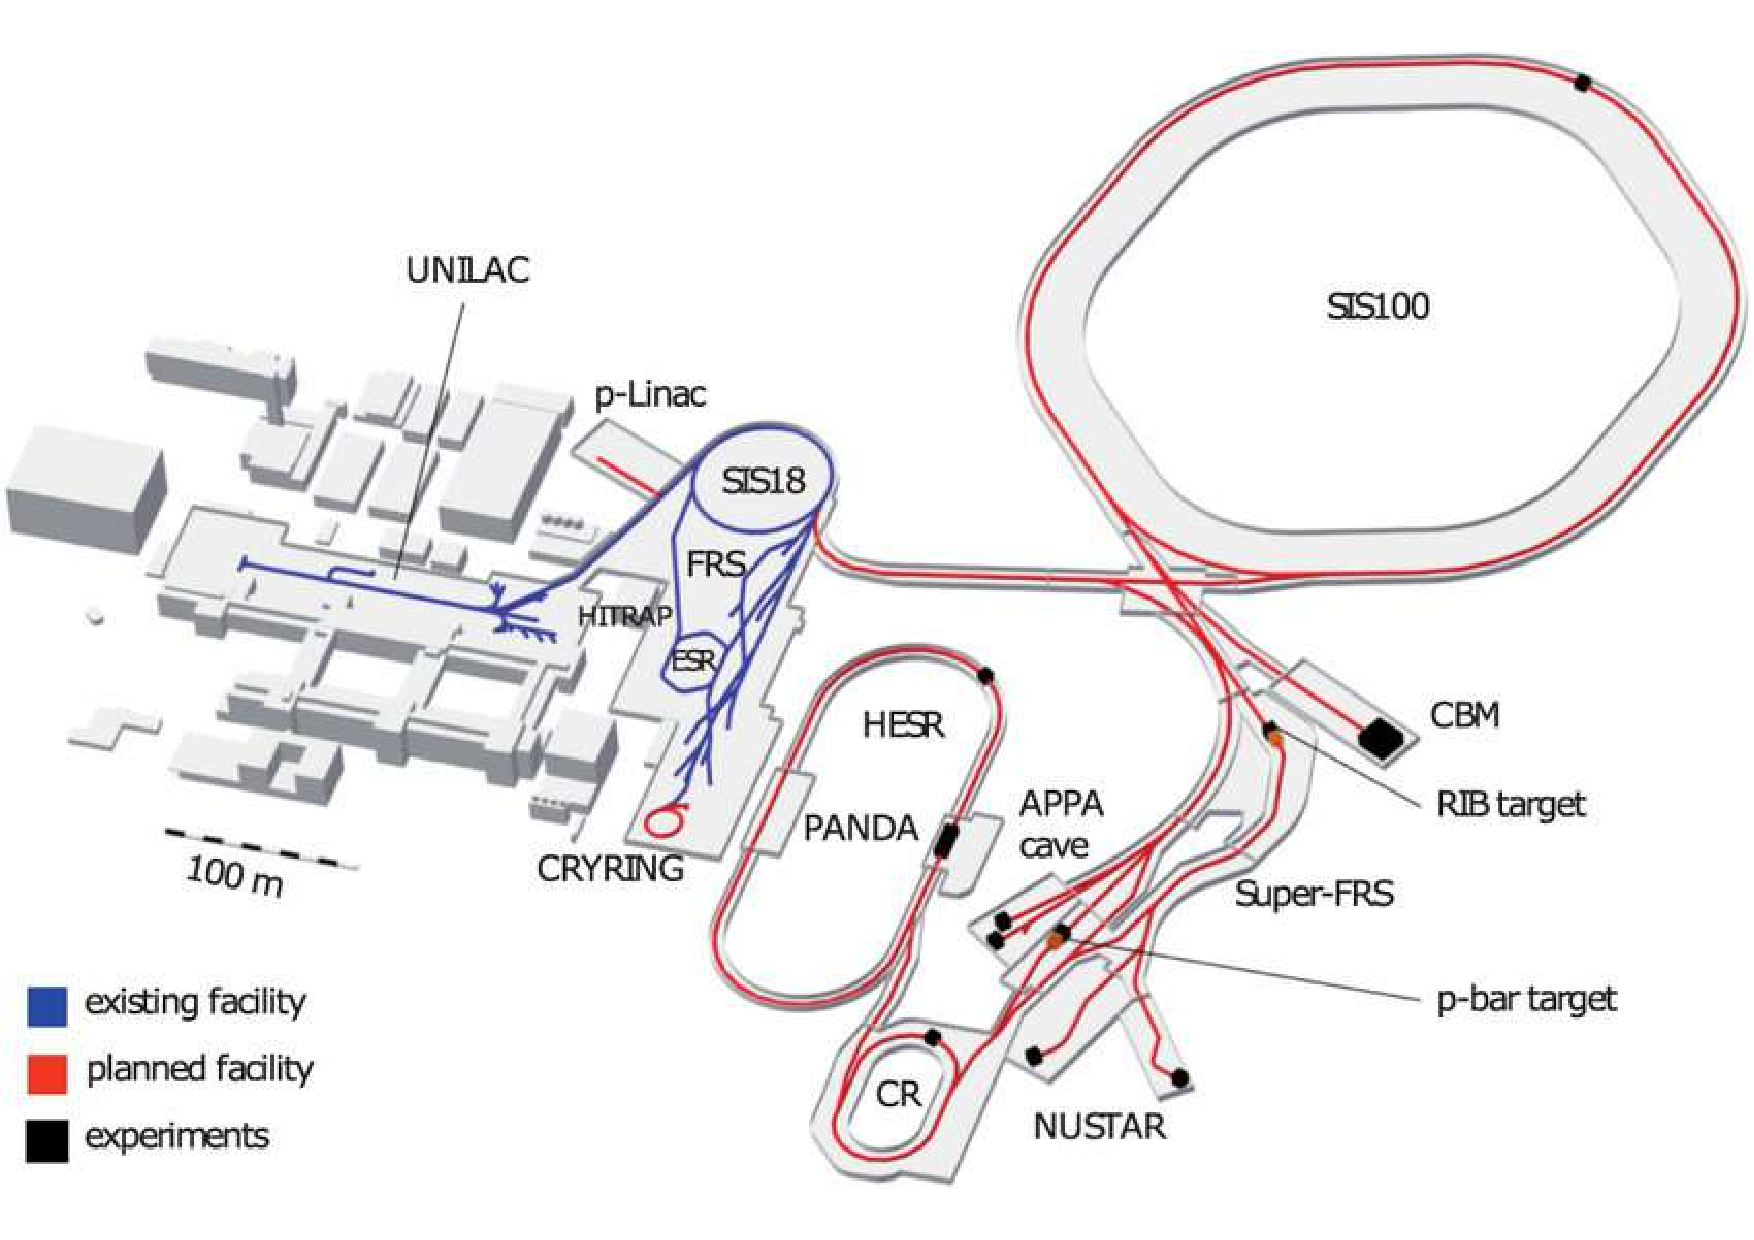
\includegraphics[width=0.75\linewidth]{FAIR}
	\caption{Layout of GSI-FAIR with the existing and planned beamlines shown in blue and red, respectively. The experimental sites are marked in black (figure: GSI Darmstadt). \textcopyright ~Copyright: GSI/FAIR.}
	\label{fig:R3BSetup}
\end{figure}


\gls{Super-FRS}

\gls{Super-FRS}

\section{Author's Contribution and Thesis Overview}
